\section{Introduction}
\begin{wrapfigure}{r}{0.4\textwidth}
\vspace{-12pt}
\centering
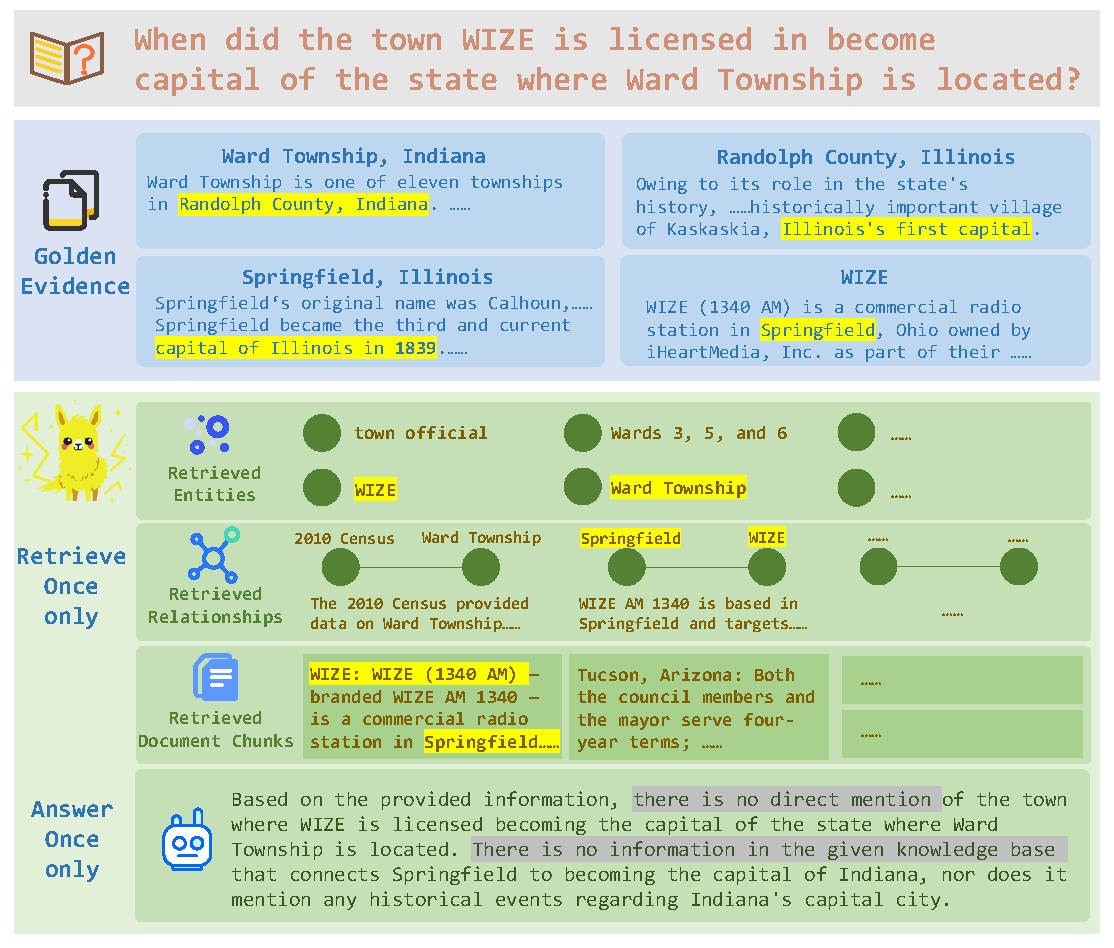
\includegraphics[width=0.4\textwidth]{figs/shallow.pdf}
\vspace{-13pt}
\caption{Shallow retrieval.}
\label{fig:challenge}
\vspace{-15pt}
\end{wrapfigure}
Large Language Models (LLMs) demonstrates remarkable capabilities in natural language understanding and reasoning~\citep{llm1,llm2}. Despite their strong performance, LLMs inherently rely on their parametric knowledge, which often results in hallucinations and a lack of factual grounding~\citep{hallucination,factuality}. Retrieval-augmented generation (RAG) has emerged as a paradigm that combines LLMs with external knowledge bases, enhancing factuality, credibility and interpretability in knowledge-intensive tasks~\citep{rag}.

More recently, Graph Retrieval-Augmented Generation (GraphRAG) is introduced to overcome the shortcomings of traditional RAG, which relies solely on semantic similarity for retrieval~\citep{graphragsurvey}. By constructing structural graph knowledge bases (graph KBs) and leveraging hierarchical retrieval strategies, GraphRAG strengthens the integration of contextual information across massive entities and relationships~\citep{raptor,graphrag,lightrag}. Building upon this foundation, some advanced graph-based enhancements that incorporate diverse structures, including heterogeneous graphs, causal graphs, and hypergraphs, to enrich representational ability and facilitate more abundant graph construction~\citep{minirag,causalrag,hypergraphrag,hyperrag,noderag}. In addition, heuristic strategies such as path-based search, pruning, and memory-inspired indexing further reinforce reasoning abilities and enable deeper multi-step exploration~\citep{pathrag,hipporag,hipporag2,proprag}.

\begin{figure}[t]
\centering
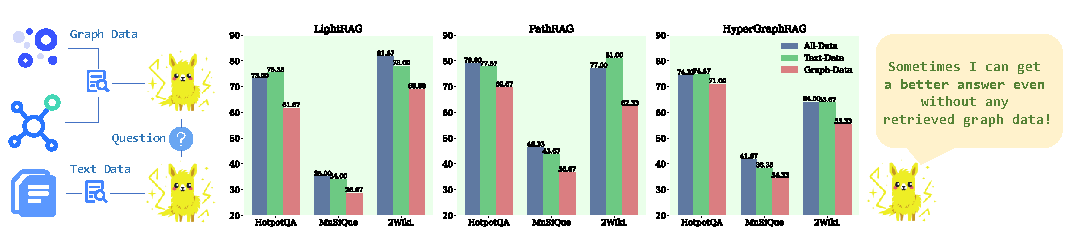
\includegraphics[width=\linewidth]{figs/rethinking.pdf}
\caption{Comparison of using graph data only, text data only, or all data as commonly adopted in GraphRAG approaches. The metric is SubEM. The contribution of retrieved graph data is marginal.}
\label{fig:rethinking}
\vspace{-10pt}
\end{figure}

However, existing GraphRAG approaches still face challenges that lead to performance bottlenecks: (i) \textbf{Shallow retrieval results in missing evidence for complex queries.} Most GraphRAG methods adopt a single-round retrieval-and-generation process as the interaction strategy between the LLM and the graph KB~\citep{graphrag, lightrag, minirag}. However, as illustrated in Figure~\ref{fig:challenge}, when handling a complex query that requires four pieces of golden evidence, \textit{``When did the town WIZE is licensed in become capital of the state where Ward Township is located?''}, the entity \textit{Randolph County} is not retrieved by the LightRAG retriever. Consequently, the LLM’s reasoning suffers from broken logic and insufficient evidence. (ii) \textbf{Limited ability to exploit structural data due to constrained retrieval scope}. Existing GraphRAG methods with heuristic path-construction schemes~\citep{minirag, pathrag, hipporag} often fail to fully leverage the structural information in graph KBs, fundamentally because shallow retrieval restricts the coverage of relevant nodes and relations. Without sufficient coverage of retrieved subgraphs, the available structural signals are fragmented and sparse, making it difficult for LLMs to integrate semantic and structural modalities for complex reasoning. As shown in Figure~\ref{fig:rethinking}, models may perform comparably with text-only evidence, highlighting that the underutilization of graph data is tightly coupled with the limitations of current retrieval strategies.

We propose \textbf{\textsc{GraphSearch}, an agentic deep searching workflow for GraphRAG}. As illustrated in Figure~\ref{fig:workflow}, \textsc{GraphSearch} is a novel agent framework designed to access graph KBs through dual-channel retrieval, acquiring both semantic and structural information, and performing multi-turn interactions to complete complex reasoning tasks. Targeting the shallow retrieval problem in existing GraphRAG approaches, \textbf{\textsc{GraphSearch} models retrieval as a modular searching pipeline}, which consists of six modules: \textit{Query Decomposition (QD)}, \textit{Context Refinement (CR)}, \textit{Query Grounding (QG)}, \textit{Logic Drafting (LD)}, \textit{Evidence Verification (EV)}, and \textit{Query Expansion (QE)}. Through the coordinated contributions of these modules, \textsc{GraphSearch} decomposes complex queries into tractable atomic sub-queries, retrieves fine-grained knowledge from graph KBs, and iteratively performs logical reasoning and reflection to remedy missing evidence. Furthermore, \textbf{\textsc{GraphSearch} adopts a dual-channel retrieval strategy}, constructing semantic queries over chunk-based text data and relational queries over structural graph data, thereby fully synergizing both modalities and integrating them into contexts that support LLMs in complex reasoning.

We conduct experiments on six multi-hop RAG datasets. The results demonstrate that leveraging the graph KBs retrievers built upon the corresponding GraphRAG approaches, \textsc{GraphSearch} consistently outperforms the single-round interaction strategy in terms of answer accuracy and generation quality, while also exhibiting strong plug-and-play capability, as shown in Table~\ref{Tab:main_exp}. Furthermore, the effectiveness of the dual-channel retrieval strategy, the contributions of agentic modules, and its robustness under a small-scale LLM and varying retrieval budgets are all empirically validated.

% Our main contributions are summarized as follows:  
% \begin{itemize}[leftmargin=*]
%     \item We propose \textsc{GraphSearch}, an agentic deep searching workflow that overcomes the challenges of shallow retrieval and the ineffective use of graph data in existing GraphRAG approaches.

%     \item We introduce a modular searching pipeline with coordinated modules for iterative reasoning and a dual-channel retrieval strategy integrating semantic and relational queries to exploit graph KBs.  

%     \item Experiment results across six multi-hop RAG datasets demonstrating that \textsc{GraphSearch} consistently outperforms vanilla GraphRAG baselines in answer accuracy and generation quality.
% \end{itemize}

% Our contributions are as follows: (i) We propose \textsc{GraphSearch}, an agentic deep searching workflow that overcomes the challenges of shallow retrieval and the ineffective use of graph data in existing GraphRAG approaches. (ii) We introduce a modular searching pipeline with coordinated modules for iterative reasoning and a dual-channel retrieval strategy integrating semantic and relational queries over graph KBs. (iii) Experiment results across six multi-hop RAG datasets demonstrating that \textsc{GraphSearch} consistently outperforms vanilla GraphRAG in accuracy and quality.